% \pgfplotsset{width=6cm}
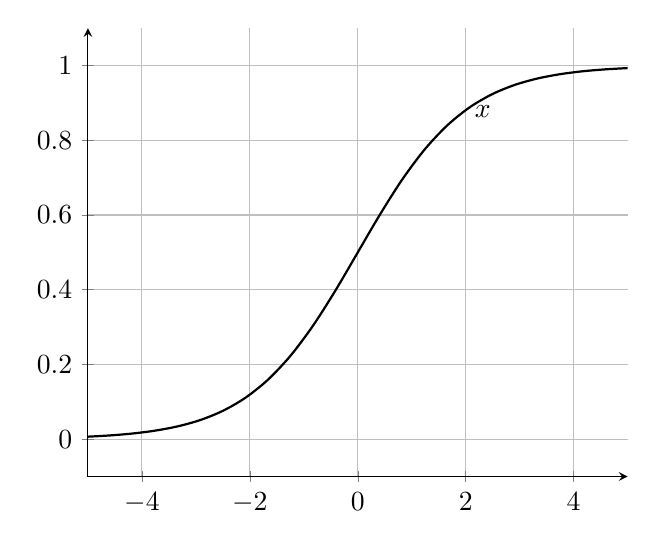
\begin{tikzpicture}
    \begin{axis}[
        % xlabel = $x$,
        % ylabel = $\sigmoid{x}$,
        ymin = -0.1,ymax = 1.1,
        domain = -6:6,
        grid=both,
        % width=5.5cm,
        smooth,
        axis lines = left,
    ]
  
    \addplot[color=black,domain=-5:5,thick]{(1+exp(-x))^(-1)} node[pos=0.7,anchor=west]{$\sigmoid{x}$};
    %   \addplot[color=blue]{tanh(x)};
    %   \addplot[color=blue,dashed,domain=-1:1,thin]{x};
        % \legend{$\sigmoid{x}$}
    \end{axis}
    % \draw (0,-1) node [inner sep=0.75pt]{
    %   $\sigmoid{x} =\frac{1}{1+e^{-x}}$
    % };
\end{tikzpicture}

% \hskip 10pt

% \begin{tikzpicture}
%     \begin{axis}[
%         xlabel = $\beta$,
%         ylabel = $\langle E\rangle/\hbar \omega$,
%         ymin = 0,ymax = 2.3,
%         domain = 0:11,
%         smooth,thick,
%         axis lines = center,
%         every tick/.style = thick]
  
%         \def\h{1}\def\w{1}
%         \def\eev{1/2*\h*\w*(1 + 4/(e^(x*\h*\w) - 1))}
%         \addplot[color=blue]{\eev};
  
%     \end{axis}
% \end{tikzpicture}
